\documentclass{urdpl}     % praca w języku polskim

% Lista wszystkich języków stanowiących języki pozycji bibliograficznych użytych w pracy.
% (Zgodnie z zasadami tworzenia bibliografii każda pozycja powinna zostać utworzona zgodnie z zasadami języka, w którym dana publikacja została napisana.)
\usepackage[english,polish]{babel}

% Użyj polskiego łamania wyrazów (zamiast domyślnego angielskiego).
\usepackage{polski}

\usepackage[utf8]{inputenc}

% dodatkowe pakiety

\usepackage[hidelinks]{hyperref}
\usepackage{float}
\usepackage{listings}
\usepackage{graphicx}
\usepackage{subcaption}
% \usepackage{booktabs} % Dla \toprule, \midrule, \bottomrule
\usepackage{multirow} 
\usepackage{tabularx} 
\usepackage{amssymb} 
\usepackage{listings}
\usepackage{xcolor}
\usepackage{array}
\usepackage{makecell}
\usepackage[flushleft]{threeparttable}
\usepackage[normalem]{ulem}
\usepackage{lineno}
\usepackage{pdfpages}
% ---------------------------------------------

% --- < bibliografia > ---

% \usepackage{csquotes}

% ------------------------
% --- < listingi > ---

% Użyj czcionki kroju Courier.
\usepackage{courier}

\usepackage{listings}
\lstloadlanguages{TeX}
\renewcommand{\lstlistlistingname}{Spis listingów}
\renewcommand{\lstlistingname}{Listing}


\lstset{
	literate={ą}{{\k{a}}}1
           {ć}{{\'c}}1
           {ę}{{\k{e}}}1
           {ó}{{\'o}}1
           {ń}{{\'n}}1
           {ł}{{\l{}}}1
           {ś}{{\'s}}1
           {ź}{{\'z}}1
           {ż}{{\.z}}1
           {Ą}{{\k{A}}}1
           {Ć}{{\'C}}1
           {Ę}{{\k{E}}}1
           {Ó}{{\'O}}1
           {Ń}{{\'N}}1
           {Ł}{{\L{}}}1
           {Ś}{{\'S}}1
           {Ź}{{\'Z}}1
           {Ż}{{\.Z}}1,
	basicstyle=\footnotesize\ttfamily,
}


% defnicja stylu JAVA
\lstdefinestyle{javaStyle}{
    language=Java,
    basicstyle=\ttfamily\footnotesize,
    keywordstyle=\color{blue},
    commentstyle=\color{green!50!black}\itshape,
    stringstyle=\color{green},
    numberstyle=\tiny\color{gray},
    numbers=left,
    numbersep=5pt,                       % Odstęp numerów od kodu
    stepnumber=1,
    showspaces=false,                    % Nie pokazuj spacji
    tabsize=2,
    showstringspaces=false,
    breaklines=true,
    breakatwhitespace=false,             % Automatyczne dzielenie wierszy
    showtabs=false,                      % Nie pokazuj tabulacji
    keepspaces=true                    % Zachowanie spacji
}


\definecolor{stringcolor}{RGB}{163,21,21}    % pomarańczowy - stringi
\definecolor{typecolor}{RGB}{43, 145, 176}     % ciemny fiolet - klasy, typy


\definecolor{lightgray}{rgb}{0.9,0.9,0.9}
    % \definecolor{blue}{rgb}{0,0,1}
    \definecolor{green}{rgb}{0,0.6,0}
    % \definecolor{red}{rgb}{0.6,0,0}
    \definecolor{gray}{rgb}{0.5,0.5,0.5}

% % ------------------------
\AtBeginDocument{
	\renewcommand{\tablename}{Tabela}
	\renewcommand{\figurename}{Rys.}   
    \newcommand{\listingname}{Listing}
}


% ------------------------
% --- < tabele > ---

% defines the X column to use m (\parbox[c]) instead of p (`parbox[t]`)
% \newcolumntype{C}[1]{>{\hsize=#1\hsize\centering\arraybackslash}X}

%---------------------------------------------------------------------------

\author{Yevhenii Usik}
\shortauthor{Y. Usik}
\noAlbum{134980}

\titlePL{Dokumentacja projektu Java na temat: "System do organizowania turniejów w DotA 2"}
\titleEN{Thesis in \LaTeX}

\shorttitlePL{Dokumentacja projektu Java na temat: "System do organizowania turniejów w DotA 2"} % skrócona wersja tytułu jeśli jest bardzo długi
\shorttitleEN{Preparation of a long and fascinating thesis in \LaTeX}

\thesistype{Praca projektowa}


\thesisDone{Praca wykonana pod kierunkiem}
\supervisor{mgr inż. Ewa Żeslawska}
%\supervisor{Jan Nowak PhD}

\degreeprogramme{Informatyka}
%\degreeprogramme{Computer Science}

\date{2025}

\department{Instytut Informatyki}
%\department{Institute of Computer Science}

\faculty{Wydział Nauk Ścisłych i Technicznych}
%\faculty{Faculty of Science and Technology}



\setlength{\cftsecnumwidth}{10mm}

%---------------------------------------------------------------------------
\setcounter{secnumdepth}{4}
\brokenpenalty=10000\relax

% --------------------------------------------------------------------------
% główna część pracy
% --------------------------------------------------------------------------

\begin{document}

\titlepages

% Ponowne zdefiniowanie stylu `plain`, aby usunąć numer strony z pierwszej strony spisu treści i poszczególnych rozdziałów.
\fancypagestyle{plain}
{
    % Usuń nagłówek i stopkę
    \fancyhf{}
    % Usuń linie.
    \renewcommand{\headrulewidth}{0pt}
    \renewcommand{\footrulewidth}{0pt}
}

\setcounter{tocdepth}{2}
\tableofcontents
\clearpage


% dodanie poszczególnych rozdziałów 

\chapter{Streszczenie}
\label{cha:streszczenie}

Ten projekt to oparta na Javie aplikacja DOTA 2 Tournament Manager zbudowana z JavaFX dla interfejsu użytkownika i Hibernate do interakcji z bazą danych. Pozwala użytkownikom widzieć krótkę najważniejszę informacje o turniejach, a także jeżeli użytkownik posiada rolę administratora, ma dodatkowe funkcji. Aplikacja zapewnia funkcje dodawania, edytowania i usuwania turniejów, a także zarządzania powiązanymi podmiotami. Schemat bazy danych został zaprojektowany do obsługi złożonych relacji między objektami, dzięki czemu nadaje się do organizowania i śledzenia wydarzeń e-sportowych DOTA 2. Projekt wykorzystuje Maven do zarządzania zależnościami i ma modułową, łatwą w utrzymaniu strukturę.


\chapter{Opis założeń Projektu}
\label{cha:opisZalozenProjektu}

\section{Cel, problem, kroki realizacji projektu}

Celem projektu jest stworzenie aplikacji do zarządzania turniejami DOTA 2, która umożliwi organizatorom kompleksowe zarządzanie danymi.  Projekt rozwiązuje problem braku wygodnego, zintegrowanego narzędzia desktopowego umożliwiającego sprawne zarządzanie danymi dotyczącymi organizacji i przebiegu turniejów e-sportowych, zwłaszcza w przypadku gry DOTA 2.  Źródłem problemu jest brak aplikacji desktopowej ze względu na trudności zarządzania wieloma powiązanymi ze sobą podmiotami, co często prowadzi do rozproszenia danych oraz trudności w ich aktualizacji i analizie.

Aby rozwiązać ten problem, konieczne było zaprojektowanie i wdrożenie aplikacji, która zapewnia centralizację danych, intuicyjny interfejs użytkownika oraz możliwość łatwego dodawania, edytowania i usuwania informacji o wszystkich kluczowych elementach turnieju. Musiałem upewnić się, że baza danych ma odpowiednią strukturę, że jest zintegrowana z graficznym interfejsem użytkownika oraz że system jest bezpieczny i wydajny.

Analiza wymagań, projektowanie bazy danych i interfejsu, implementacja funkcjonalności, testowanie i wdrożenie to kroki, które zostały podjęte w ramach projektu.

\section{Wymagania:}
\subsection{Funkcjonalne}

\begin{itemize}
    \item Możliwość dodawania, edytowania i usuwania turniejów.
    \item Przeglądanie listy turniejów oraz szczegółowych informacji o każdym z nich.
    \item Autoryzacja użytkowników i zarządzanie poziomami dostępu.
    \item Wybór typu turnieju (jeżeli offline - trzeba wprowadzić lokalizację) i organizatora turnieju z listy dostępnych (tylko dla administratora).
\end{itemize}
\subsection{Niefunkcjonalne}
\begin{itemize}
    \item Intuicyjny, z odpowiednią estetyką (temat DOTA2) interfejs.
    \item Bezpieczeństwo przechowywanych danych (uwierzytelnianie, autoryzacja, hashowanie haseł).
    \item Łatwość utrzymania i rozbudowy systemu.
    \item Łatwość wprowadzania zmian w bazie danych i aplikacji.
\end{itemize}

\chapter{Opis struktury Projektu}
\label{cha:opisStrukturyProjektu}


\section{Cała Struktura Projektu}
\begin{figure}[h!]
    \centering
    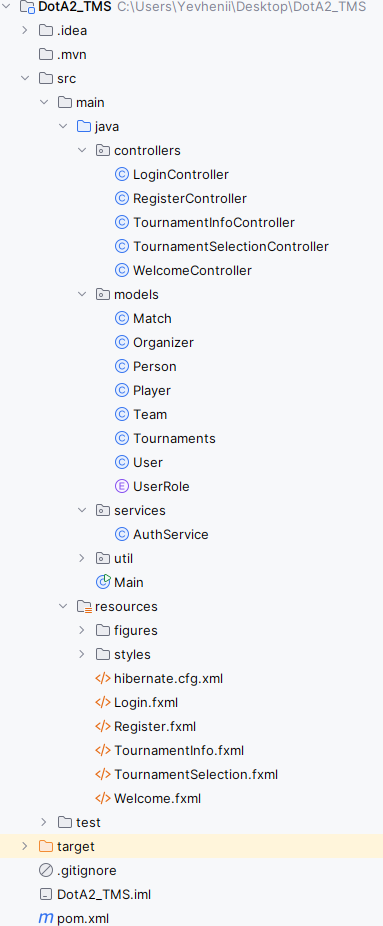
\includegraphics[width=0.5\textwidth]{figures/Structure.png}
    \caption{Struktura całego projektu \label{fig1}}
\end{figure}
\begin{figure}[h!]
    \centering
    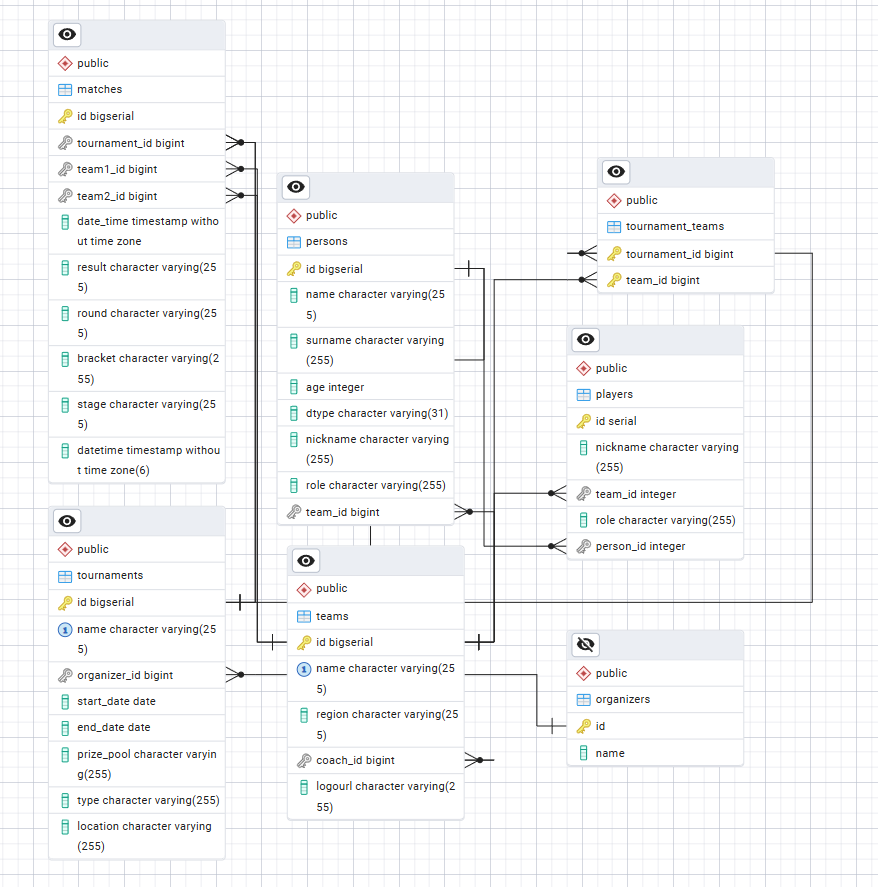
\includegraphics[width=0.8\textwidth]{figures/Database.png}
    \caption{Baza danych \label{fig2}}
\end{figure}

\subsection{Main}

Main po prostu uruchamia aplikacje i ustawia ikonę i title dla programu, zaczyna się ona od \texttt{Welcome.fxml}(interfejs zademonstruje w następującym rozdziale).

\lstinputlisting[caption= Main: jak zaczyna się program, label=JavaListing, style = javaStyle, firstline=8, lastline=24]{src/Main.java}


\subsection{Util and Service}
\lstinputlisting[caption= Klasa HibernateUtil: odpowiedzialna za konfigurację bazy danych, label=JavaListing, style = javaStyle, firstline=5]{src/HibernateUtil.java}

\lstinputlisting[caption= Klasa AuthService: autoryzacja z wyszukiwaniem w bazie konta i dehashowaniem hasła BCryptem, label=JavaListing, style = javaStyle, firstline=17, lastline=34]{src/AuthService.java}

\lstinputlisting[caption= Klasa AuthService: rejestracja ze sprawdzeniem czy istnieje już konto i hashowanie hasła nowego użytkownika, label=JavaListing, style = javaStyle, firstline=44, lastline=66]{src/AuthService.java}

\subsection{Controllers}
Pakiet \texttt{controllers} zawiera klasy odpowiedzialne za backend fxml plików. 

\begin{figure}[H]
    \centering
    \caption{Metody kontrolerów \label{fig4}}
    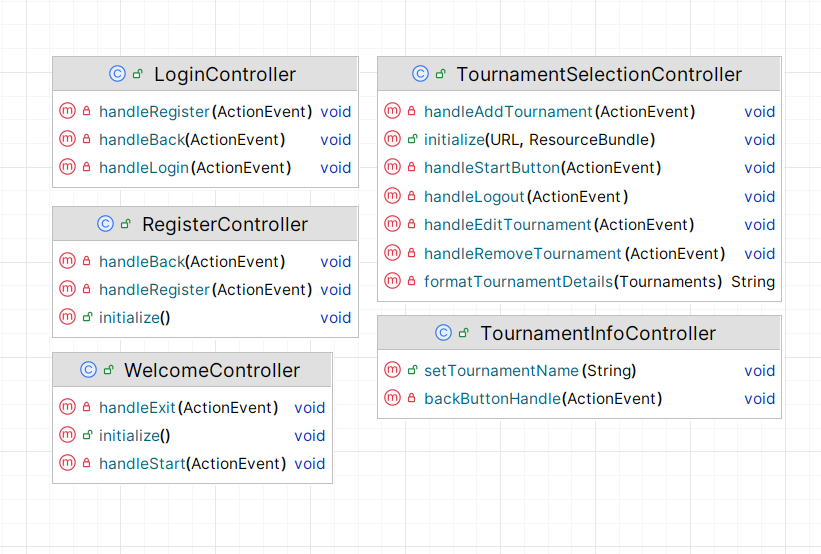
\includegraphics[width=0.8\textwidth]{figures/ControllersMethods.png}
\end{figure}

\lstinputlisting[caption= Klasa LoginController: handleBack i handleRegister - przekazania na nowe strony; handleLogin - logowanie użytkownika z wykorzystaniem wyżej opisanym AuthService dla autentyfikacji usera i przy poprawnych danych - przekazanie na nową stronę, label=JavaListing, style = javaStyle, firstline=32, lastline=92]{src/LoginController.java}

\lstinputlisting[caption= Klasa RegisterController: handleRegister - rejestracja nowego użytkownika z wykorzystaniem AuthService; umożliwia rejestrację jako Admin za pomocy sprawdzenia adminCodeField (admin code = 1111); obsługuje już istniejące lub puste dane, label=JavaListing, style = javaStyle, firstline=27, lastline=86]{src/RegisterController.java}

\lstinputlisting[caption= Klasa TournamentSelectionController: w tej klasie przy inicjalizację jest kontrola roli użytkownika i zrealizowane CRUD na turniejach(używamy HibernateUtil opisany wyżej); W przyszłości ulepszę tę klasę, label=JavaListing, style = javaStyle, firstline=68, lastline=418]{src/TournamentSelectionController.java}


\subsection{Models}

Pakiet \texttt{models} zawiera klasy, które są mapowane na tabele w bazie danych.

\begin{figure}[H]
    \centering
    \caption{Pola i dziedziczenie klas, każda klasa ma gettery i settery, a także metodę ToString  \label{fig3}}
    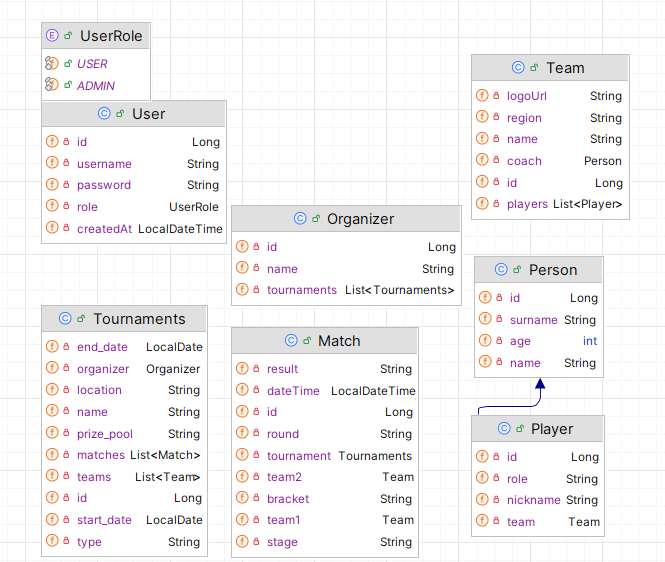
\includegraphics[width=0.8\textwidth]{figures/Classes.png}
\end{figure}

\lstinputlisting[caption= Przykład mapowania klas na klasie Tournaments, label=JavaListing, style = javaStyle, firstline=8, lastline=42]{src/Tournaments.java}

\subsection{Resources}
Pakiet \texttt{resources} zawiera pliki fxml, które są odpowiedzialne za wygląd aplikacji. Każdy plik jest rozpatrzony w następnym rozdziale.

Zawiera plik css, który daje ten ładny wygląd aplikacji, jest on wykorzystywany w każdym pliku fxml, aby zapewnić spójność stylu. Jest folder figures z obrazkami.

\section{Wykorzystane Technologie}
W projekcie wykorzystano następujące technologie:
\begin{itemize}
    \item \textbf{IntelliJ IDEA 2025.1.2} - IDE do tworzenia aplikacji w języku Java.
    \item \textbf{Maven 4.0.0} - budowanie projektu i zarządzanie zależnościami.
    \item \textbf{JavaFX 21.0.7} - projektowanie GUI.
    \item \textbf{JavaFX SceneBuilder} - projektowanie GUI.
    \item \textbf{PostgreSQL 17.5} - baza danych.
    \item \textbf{Hibernate 6.2.7} - warstwa ORM.
    \item \textbf{BCrypt} - bezpieczne hashowanie haseł.
\end{itemize}

\subsection{Wymagania sprzętowe}
Aby uruchomić aplikację, wymagany jest komputer z systemem operacyjnym Windows 10/11, Intellij Idea, Java 21, PostgreSQL i JavaFX 21.0.7.

Wszystko trzeba poprawnie skonfigurować, aby aplikacja działała poprawnie. W razie potrzeby wrzucę filmik z instrukcją repozytorium.


\chapter{Harmonogram Realizacji Projektu}
\label{cha:harmonogramRealizacjiProjektu}

Najtrudniejszym było zapoznać się z nowymi technologiami, takimi jak JavaFX i Hibernate, oraz LaTeX, ponieważ wcześniej pracowałem głównie z JDBC i Swing. Jednakże, dzięki książkom, tutorialom na YouTube, stackoverflow, udało mi się szybko opanować podstawy tych technologii.

Odpowiednio do wymagań, stworzyłem diagram Gantta, który widziano poniżej:

\begin{figure}[h!]
    \centering
    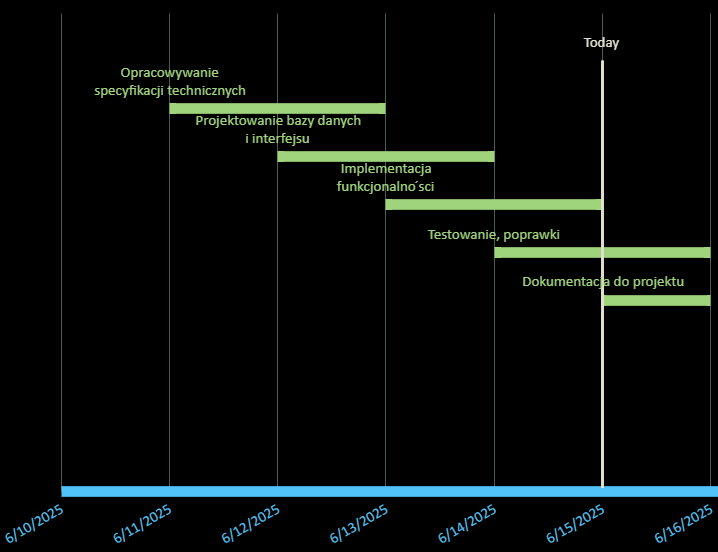
\includegraphics[width=0.8\textwidth]{figures/Gantt.png}
    \caption{Diagram Gantta \label{fig2}}
\end{figure}

\subsection{Repozytorium}

Kod źródłowy projektu jest dostępny w repozytorium GitHub pod adresem: \url{https://github.com/kayor1x/ProjectJava1rok}


\chapter{Prezentacja warstwy użytkowej projektu}
\label{cha:PrezentacjaGUI}

\section{Welcome.fxml}

Pierwszy ekran, można nacisnąć exit i wyjść lub start i zacząć logowanie.
\begin{figure}[H]
    \centering
    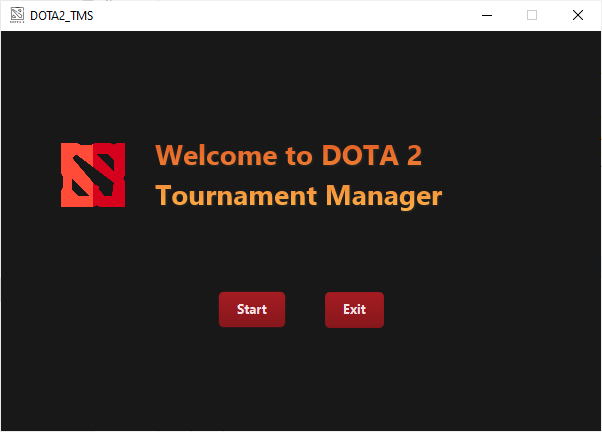
\includegraphics[width=0.5\textwidth]{figures/Welcome.png}
    \caption{Ekran powitalny \label{fig:welcome}}
\end{figure}

\section{Login.fxml}
Ekran logowania, gdzie można się zalogować lub zarejestrować lub wrócić do ekranu powitalnego.
\begin{figure}[H]
    \centering
    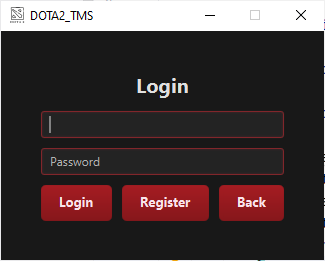
\includegraphics[width=0.5\textwidth]{figures/Login1.png}
    \caption{Ekran logowania \label{fig:login}}
\end{figure}
\begin{figure}[H]
    \centering
    \begin{subfigure}{0.7\linewidth}
        \centering
        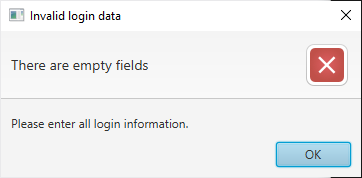
\includegraphics[width=.6\linewidth]{figures/FailedLogin1.png}
    \end{subfigure}
    \begin{subfigure}{0.7\linewidth}
        \centering
        \subcaption{\label{subfigure_a}}
        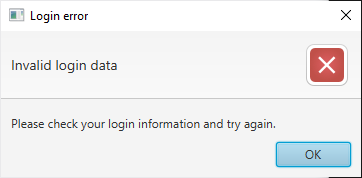
\includegraphics[width=.6\linewidth]{figures/FailedLoginData.png}
        \subcaption{\label{subfigure_b}}
    \end{subfigure}
    \begin{subfigure}{0.7\linewidth}
        \centering
        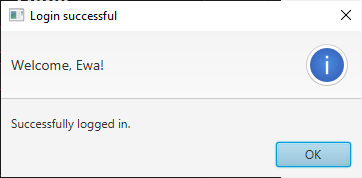
\includegraphics[width=.6\linewidth]{figures/SuccesLogin.png}
        \subcaption{\label{subfigure_c}}
    \end{subfigure}
    \caption{ Błedne i Udane logowania: \protect\subref{subfigure_a} Empty fields error, \protect\subref{subfigure_b} Invalid login data(nieznaleziono w db), \protect\subref{subfigure_c} Successful login. \label{fig:subcaption}}
\end{figure}
\section{Register.fxml}
Ekran rejestracji, gdzie można się zarejestrować lub wrócić do ekranu logowania. Przy logowaniu możesz wybrać rolę.
\begin{figure}[H]
    \centering
    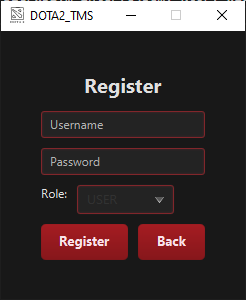
\includegraphics[width=0.4\textwidth]{figures/Register1.png}
    \caption{Ekran rejestracji z wybranym User \label{fig:register}}
\end{figure}
\begin{figure}[H]
    \centering
    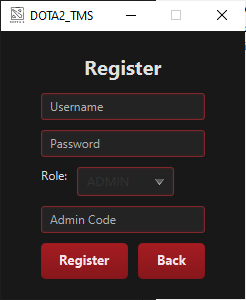
\includegraphics[width=0.4\textwidth]{figures/Register2.png}
    \caption{Ekran rejestracji z wybranym Admin \label{fig:register1}}
\end{figure}
\begin{figure}[H]
    \begin{subfigure}{0.5\textwidth}
        \centering
        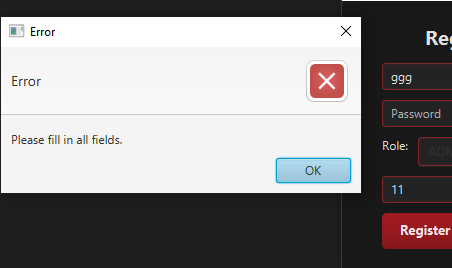
\includegraphics[width=.7\linewidth]{figures/ErrorFields.png}
        \subcaption{\label{subfigure_a}}
    \end{subfigure}
    \begin{subfigure}{0.5\textwidth}
        \centering
        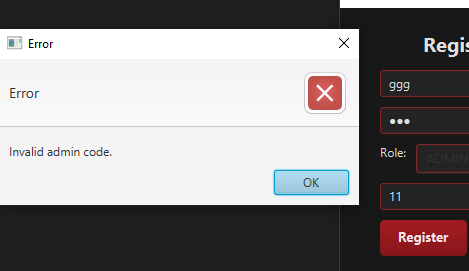
\includegraphics[width=.7\linewidth]{figures/ErrorCode.png}
        \subcaption{\label{subfigure_b}}
    \end{subfigure}
    \begin{subfigure}{0.5\textwidth}
        \centering
        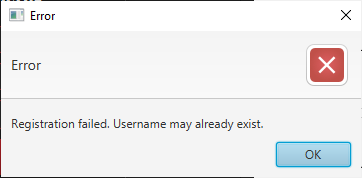
\includegraphics[width=.7\linewidth]{figures/ErrorExist.png}
        \subcaption{\label{subfigure_c}}
    \end{subfigure}
    \begin{subfigure}{0.5\textwidth}
        \centering
        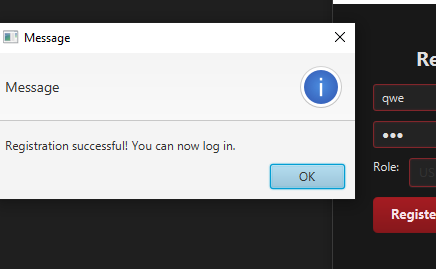
\includegraphics[width=.7\linewidth]{figures/SuccesRegister.png}
        \subcaption{\label{subfigure_d}}
    \end{subfigure}
    \caption{ Błedne i Udane rejestracji: \protect\subref{subfigure_a} Empty fields error, \protect\subref{subfigure_b} Invalid admin code, \protect\subref{subfigure_c} User already exists, \protect\subref{subfigure_d} Successful registration. \label{fig:subcaption}}
\end{figure}

\section{TournamentSelection.fxml}
Ekran wyboru turnieju, gdzie można wybrać dostępny turniej lub wylogować się i wrócić do ekranu logowania. Jeżeli jesteś adminem, możesz dodać, edytować lub usunąć turniej.\begin{figure}[H]
    \centering
    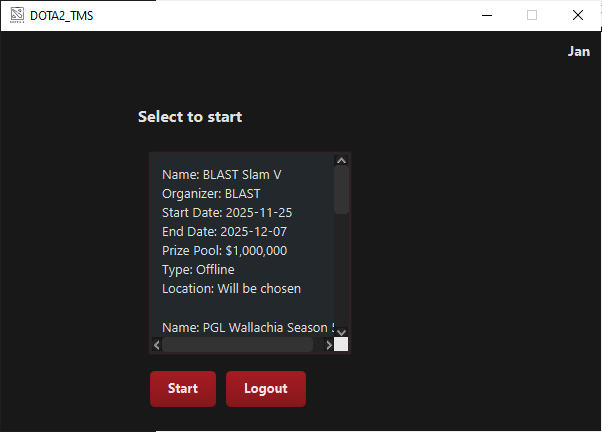
\includegraphics[width=0.4\textwidth]{figures/UserInterface.png}
    \caption{Ekran wyboru turnieju jako User \label{fig:tournament_selection}}
\end{figure}
\begin{figure}[H]
    \centering
    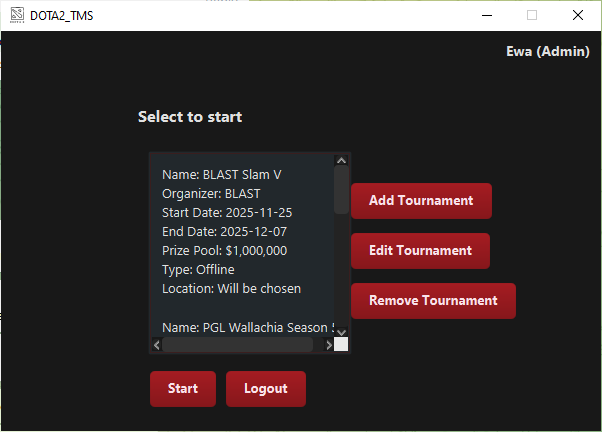
\includegraphics[width=0.4\textwidth]{figures/AdminInterface.png}
    \caption{Ekran wyboru turnieju jako Admin \label{fig:tournament_selection_admin}}
\end{figure}
\begin{figure}
    \centering
    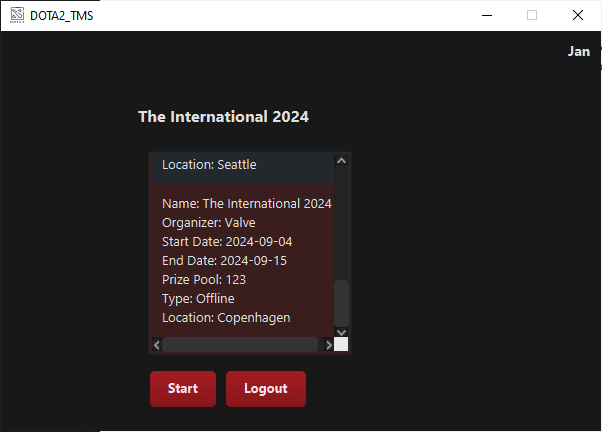
\includegraphics[width=0.4\textwidth]{figures/Chosen.png}
    \caption{Gdy klikasz na turniej górny label zmienia się \label{fig:tournament_selection_fxml}}
\end{figure}
\begin{figure}
    \centering
    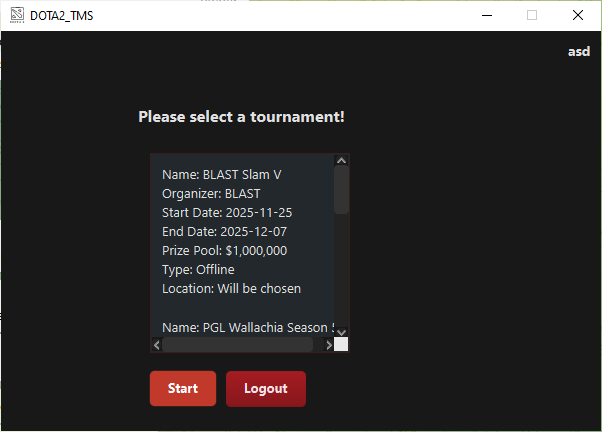
\includegraphics[width=0.4\textwidth]{figures/IfPressStart.png}
    \caption{Gdy klikasz start, prosi o wyborze turnieju \label{fig:tournament_selection_fxml_admin}}
\end{figure}
\begin{figure}[H]
    \centering
    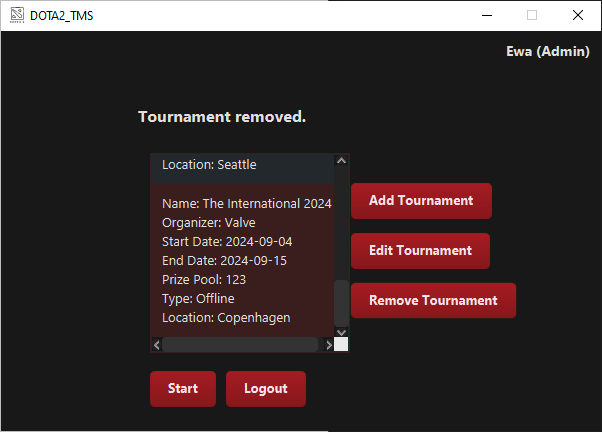
\includegraphics[width=0.4\textwidth]{figures/Removing.png}
    \caption{Gdy klikasz remove, wyrzuca go z bazy danych i tabeli, zmienia się górny label \label{fig:tournament_selection_fxml_remove}}
\end{figure}
\begin{figure}
    \centering
    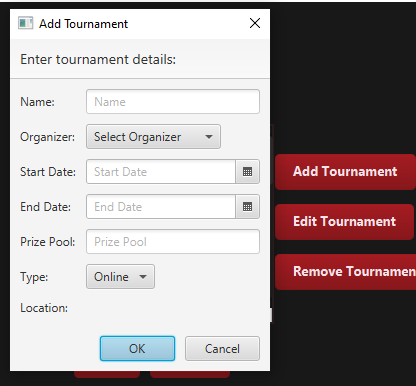
\includegraphics[width=0.4\textwidth]{figures/Add.png}
    \caption{Gdy klikasz add, otwiera się okno z formularzem do dodania turnieju \label{fig:tournament_selection_fxml_add}}
\end{figure}
\begin{figure}[H]
    \begin{subfigure}{0.3\textwidth}
        \centering
        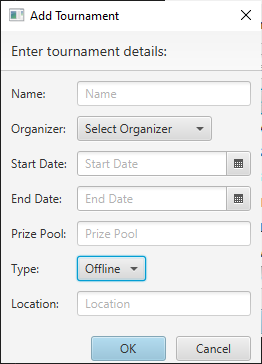
\includegraphics[width=.8\linewidth]{figures/AddOffline.png}
        \caption{Typ offline, pojawia sie miejsce prowadzenia \label{subfigure_name}}
    \end{subfigure}
    \begin{subfigure}{0.3\textwidth}
        \centering
        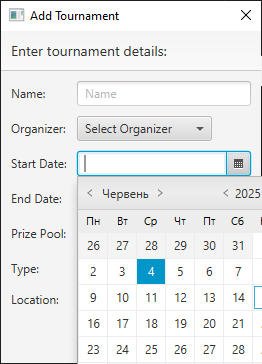
\includegraphics[width=.8\linewidth]{figures/SelectingData.png}
        \caption{Możesz wybrać dowolną datę rozpoczęcia turnieju \label{fig:tournament_selection_fxml_edit}}
    \end{subfigure}
    \begin{subfigure}{0.3\textwidth}
        \centering
        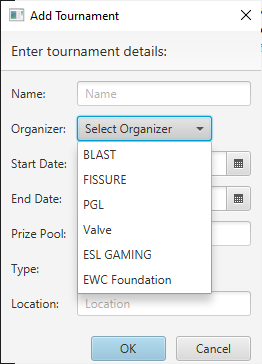
\includegraphics[width=.8\linewidth]{figures/SelectingOrganizer.png}
        \caption{Możesz wybrać organizatora turnieju \label{fig:tournament_selection_fxml_add_offline}}
    \end{subfigure}
    \caption{Formularz do dodania lub edycji turnieju: \protect\subref{subfigure_name}, \protect\subref{fig:tournament_selection_fxml_edit}, \protect\subref{fig:tournament_selection_fxml_add_offline}. \label{fig:tournament_selection_fxml_form}}
\end{figure}
\begin{figure}[H]
    \begin{subfigure}{0.6\textwidth}
        \centering
        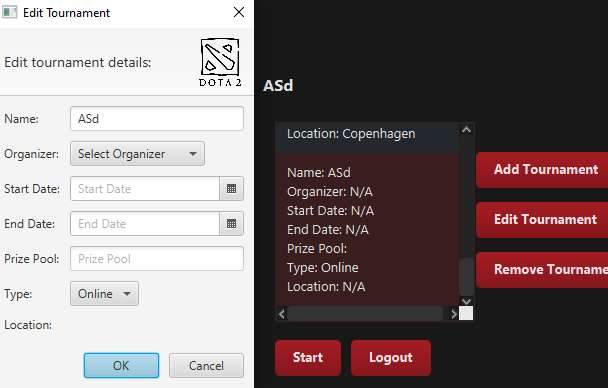
\includegraphics[width=.8\linewidth]{figures/Edit.png}
        \caption{Przy edycje już wprowadzone dane wypełniają odpowiene pola \label{subfigure_name}}
    \end{subfigure}
    \begin{subfigure}{0.6\textwidth}
        \centering
        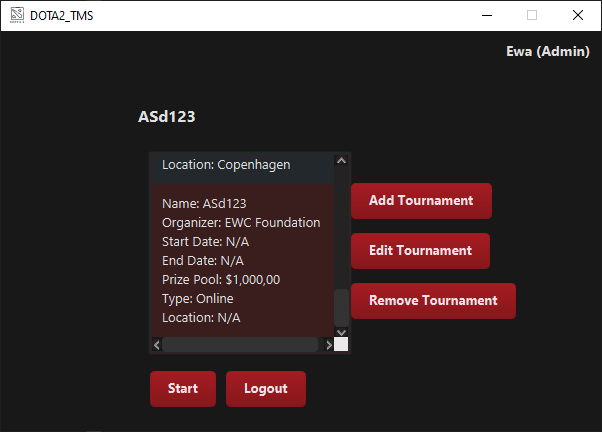
\includegraphics[width=.8\linewidth]{figures/Edited.png}
        \caption{Wprowadziłem jakieś zmiany w formularzu \label{fig:tournament_selection_fxml_edit}}
    \end{subfigure}
    \caption{Edycja turnieju: \protect\subref{subfigure_name}, \protect\subref{fig:tournament_selection_fxml_edit}. \label{fig:tournament_selection_fxml_edit_form}}
\end{figure}
\section{TournamentInfo.fxml}
Ekran informacji o turnieju, nie ma jeszcze żadnych odpowiednich funkcji, tylko Back żeby wrócić do wyboru.
\begin{figure}[H]
    \begin{subfigure}{0.6\textwidth}
        \centering
        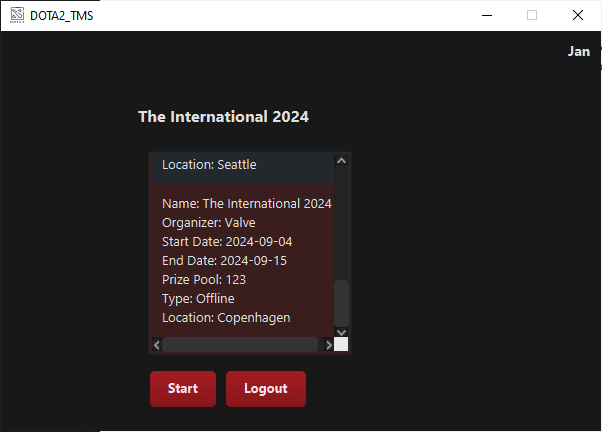
\includegraphics[width=.8\linewidth]{figures/Chosen.png}
        \caption{Wybieram jakiś turniej \label{subfigure_name}}
    \end{subfigure}
    \begin{subfigure}{0.6\textwidth}
        \centering
        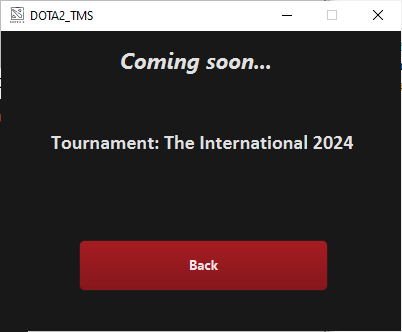
\includegraphics[width=.7\linewidth]{figures/Info.png}
        \caption{W przyszłości planowane są dodatkowe funkcje \label{fig:tournament_selection_fxml_edit}}
    \end{subfigure}
    \caption{Ekran informacji o turnieju: \protect\subref{subfigure_name}, \protect\subref{fig:tournament_selection_fxml_edit}. \label{fig:tournament_selection_fxml_edit_form}}
\end{figure}
\chapter{Podsumowanie}
\label{cha:podsumowanie}

Ten projekt jest moim pierwszym projektem w ogóle, zdecydowałem się zaimplementować go w JavaFX i Hibernate, z którymi jestem mniej zaznajomiony, ponieważ w laboratoriach używaliśmy JDBC i Swing, które moim zdaniem są łatwiejsze. Ale tak czy inaczej, do tej pory zaimplementowałem następujące funkcje:
\begin{itemize}
    \item Wygodny i odpowiadający tematowi DOTA 2 interfejs użytkownika.
    \item Rejestracja, logowanie użytkowników.
    \item Zarządzanie poziomami dostępu.
    \item Haszowanie haseł użytkowników w bazie danych.
    \item Dodawanie, edytowanie i usuwanie turniejów (wszystko jest połączone z db).
    \item Przeglądanie listy turniejów oraz szczegółowych informacji o każdym z nich.
    \item Wybór typu turnieju (jeżeli offline - trzeba wprowadzić lokalizację) i organizatora turnieju z listy dostępnych (tylko dla administratora).
\end{itemize}

W przyszłości planuję dodać więcej funkcji, takich jak:
\begin{itemize}
    \item Po wyborze turnieju, zwiększyć funkcjonalności dla użytkownika widzieć informacje o drużynach, graczach, meczach tego turnieju.
    \item Dla administratora możliwość zarządzania wszystkimi aspektami turnieju.
    \item Dodać możliwość przeglądania nowości o turniejach DOTA 2(web integracja).
    \item Ulepszenie już zrobionych funkcji.
\end{itemize}

% Wyłączenie działania `ulem` na czas bibliografii
\renewcommand{\emph}[1]{\textit{#1}}
% Bibliografia
% Dodanie bibliografi do spisu treści
% \addcontentsline{toc}{section}{\textbf{Bibliografia}}
% \bibliographystyle{plain}
% \bibliography{bibliografia}

% Przywrócenie działania `ulem`
\renewcommand{\emph}[1]{\uline{#1}}

\clearpage
% Dodanie spisu rysunków do spisu treści
\addcontentsline{toc}{section}{\textbf{Spis rysunków}}
\listoffigures
\clearpage



\clearpage

% Dodanie spisu listingow do spisu treści
\addcontentsline{toc}{section}{\textbf{Spis listingów}}
\lstlistoflistings
\clearpage



\includepdf[pages=-]{appendix/oswiadczenie.pdf}

\end{document}
